
\section{Entscheidung}
Die zur Auswahl stehenden Systeme sind NuPRL, Coq und Idris, wobei es sich bei Coq und NuPRL um interaktive Beweissysteme auf Basis vom ML handelt. Idris ist an die Haskell Syntax angelehnt ist. In allen drei Systemen stehen Taktiken zur Beweisf\"uhrung und zur Verbesserung der Lesbarkeit zur Verf\"ugung und es handelt sich um funktionale Programmiersprachen h\"oheren Levels. %Formulierung 

In den Systemen NuPRL und Coq gibt es bereits erste Realisierungen von Automaten. Die NuPRL Realisierung ist aus dem Jahr 1986 \cite{Krei86} und k\"onnte als Ideengeber angesehen werden, da sich das System mit der Zeit stark ver\"andert hat.  %Formulierung

Die NuPRL Architektur besteht aus einer Wissensbasis als Zentrum, die durch die Nutzer stetig erweitert werden kann, und anliegenden Schnittstellen, wie beispielsweise der Benutzeroberfl\"ache. Sie bietet ebenfalls automatische Tools wie Entscheidungsprozeduren, Theorembeweiser, Beweisplaner, Modelchecker, Rewrite Enginges an. %Formulierung

\begin{figure}[h!] %  figure placement: here, top, bottom, or page
   \centering
   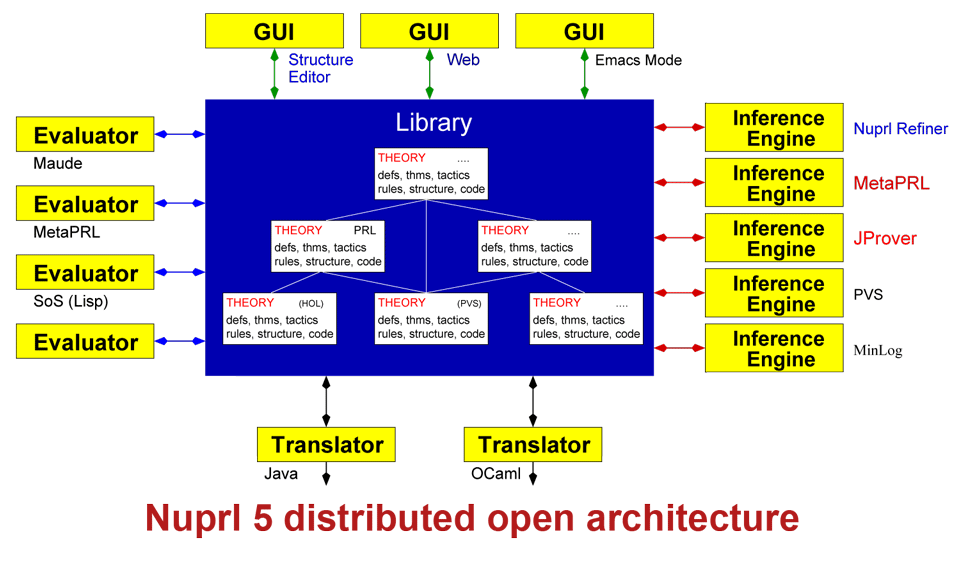
\includegraphics[width=1.0\textwidth]{NuPRL-Architiktur.PNG} 
   \caption{NuPRL 5 Architektur \cite{Nu5arch}}
   \label{fig:example}
\end{figure}

Verschiedene Nutzer k\"onnen parallel auf die Wissensbasis zugreifen und alle \"Anderungen werden umgehend \"ubertragen, so dass im Falle eines Systemausfalls beim Benutzer, keine Daten verloren gehen. Bei \"Anderungen an Objekten werden diese nicht \"uberschrieben sondern es wird eine neue Version vom jeweiligen Objekt erstellt. Dieses Vorgehen erm\"oglicht es, \"altere Versionen wieder herzustellen um somit beispielsweise mehrere Beweise eines Theorems zu erstellen. 

Die Komplexit\"at des Systems mit den vielen Schnittstellen und den verschiedenen graphischen Darstellungsm\"oglichkeiten f\"ur den Benutzer erscheint am Anfang sehr un\"ubersichtlich und der Code ist nicht unbedingt intuitiv lesbar. %zu komplex f�r Einsteiger

%- \begin{quotation}
%   The Nuprl LPE (logical programming environment) is an open , distributed architecture that integrates all its key subsystems as independent components and, by using a flexible knowledge base as its central component, supports the interoperability of current proof technology.
%  \end{quotation}

Die Realisierungen von endlichen Automaten in Coq sind deutlich j\"unger. So wird ein Formalismus zur Darstellung von regul\"aren Ausdr\"ucken im Jahr 2011 beschrieben \cite{RA2011}. Es gibt eine ganze Reihe von Ans\"atzen, die in dieser Arbeit betrachtet und bez\"uglich ihrer Verwendbarkeit analysiert werden.

Coq ist ein intuitionistischer Theorembeweiser mit einer einfach strukturierten Benutzeroberfl\"ache, der CoqIDE. Es gibt diverse Online Tutorials zur Installation und Anwendung \cite{TuCoq}. Die dem System zugrundeliegende Theorie ist der \glqq Calculus of Inductive Constructions\grqq{} \cite[S. V]{CoqBuch}. Weiterhin werden Exporte in g\"anginge Formate, wie XML, HTML und \LaTeX angeboten \cite{Export}. Die aktive Gemeinschaft u.a. in Form einer Mailing Liste, reagiert schnell auf Fragen und ist leicht zug\"anglich \cite{Mail}.
 
Idris bietet ebenfalls ein funktionales Interface, welches die Interaktion mit einer externen C Bibliothek erm\"oglicht. Die Verwendung der Taktik basierten Beweisf\"uhrung wurde von Coq beeinflusst \cite{IdCoq}. Eine aktive Gemeinschaft ist ebenfalls u.a. in Form einer Mailing Liste gegeben \cite{MailIdris}. Exporte sind u.a. in Javascript m\"oglich \cite{IdrisTutorial}. Allerdings bietet Idris von sich aus keine Benutzeroberfl\"ache und kann entweder \"uber Vim oder Emacs benutzt werden \cite{IdrisIDE}. Weiterhin muss man beim Programmieren beachten, dass gewisse Argumente exakt untereinander stehen, da es sonst zu Problemen f\"uhren kann \cite{IdrisTutorial}.
%gibt es die ? Variante, wenn ein Beweis noch nicht komplett gef�hrt wurde auch in Coq?
 
Ein weiterer wichtiger Aspekt f\"ur die sp\"atere Anwendung ist eine einfache Installation des zugrundeliegenden Systems unabh\"agig vom Betriebssystem. Dies ist sowohl bei Coq, als auch bei Idris gegeben. NuRPL l\"auft nur \"uber eine virtuelle Maschine und Installationsinformationen sind nur sehr schwer zu finden.

Coq und Idris sind zwei Systeme, die im Moment von zwei aktiven Communities gepflegt und weiterentwickelt werden. Die aktuelle Coq Version 8.4pl5 wurde am 31.10.2014 ver\"offentlicht \cite{Coq84} und die 8.5 beta 1 Version kam am 21.01.2015 \cite{Coq85}. Bei Idris erschien das letzte Release 0.9.16 am 15. Januar 2015 \cite{IdRel}. Im Gegensatz dazu ist bei NuPRL das letzte Release, NuPRL 5, 2000 erschienen \cite{Nu5}. Aus diesem Grund und wegen der Probleme bei dem Beziehen der Plattform und der Installationsprobleme klammere ich NuPRL aus meinen weiteren Betrachtungen aus.

